\documentclass{article}
\usepackage{CJK}
\usepackage{amsmath}
\usepackage{amsthm}
\usepackage{amsfonts}
\usepackage{palatino}
\usepackage{xcolor}
\usepackage{geometry}
\usepackage{listings}
\usepackage{pxfonts}
\usepackage{enumerate}
\usepackage[pdftex]{graphicx}
\geometry{left=2cm,right=2cm,top=3cm,bottom=3cm}
\pagestyle{myheadings}
\markright{Huiqian Yu/14300180118}
\setlength{\parindent}{0pt}
\newcommand{\ix}[1]{\intertext{{}#1}}
\newcommand{\dx}{\;\mathrm{d}\,x}
\newcommand{\dt}{\;\mathrm{d}\,t}
\newcommand{\dm}[1]{\;\mathrm{d}\,{}#1}
\newcommand{\ve}{\varepsilon}
\newcommand{\tp}{^\mathsf{T}}
\newcommand{\var}{\mathrm{var}}
\newcommand{\corr}{\mathrm{corr}}
\newcommand{\mbe}[1]{\mathbb{E}\left[{}#1\right]}
\newcommand{\argmin}[1]{\mathop{\arg\min}_{{}#1}}
\begin{document}

\definecolor{backcolour}{rgb}{0.95,0.95,0.92}
\begin{CJK*}{GBK}{song}
\begin{enumerate}
\item[3.9]
The plots is as follows. The plot is not so good because of white noise. If we sample more data, like $n=1000$, which is shown below, it fits Table~3.1 better.
\begin{center}
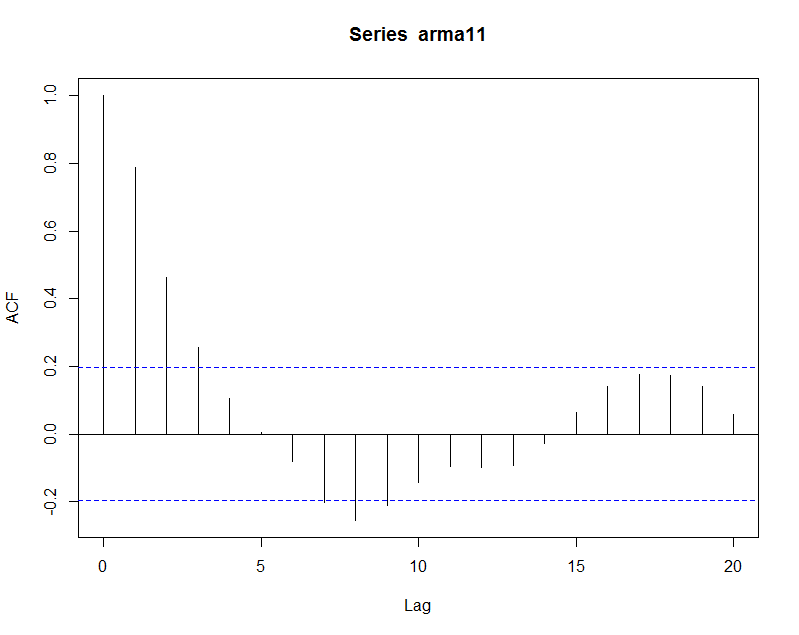
\includegraphics[width=5cm]{1.png}
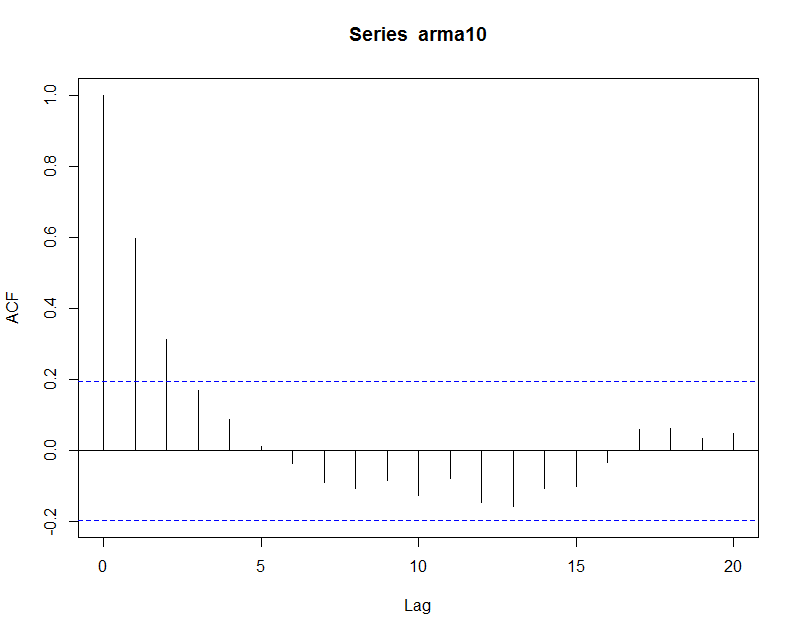
\includegraphics[width=5cm]{2.png}
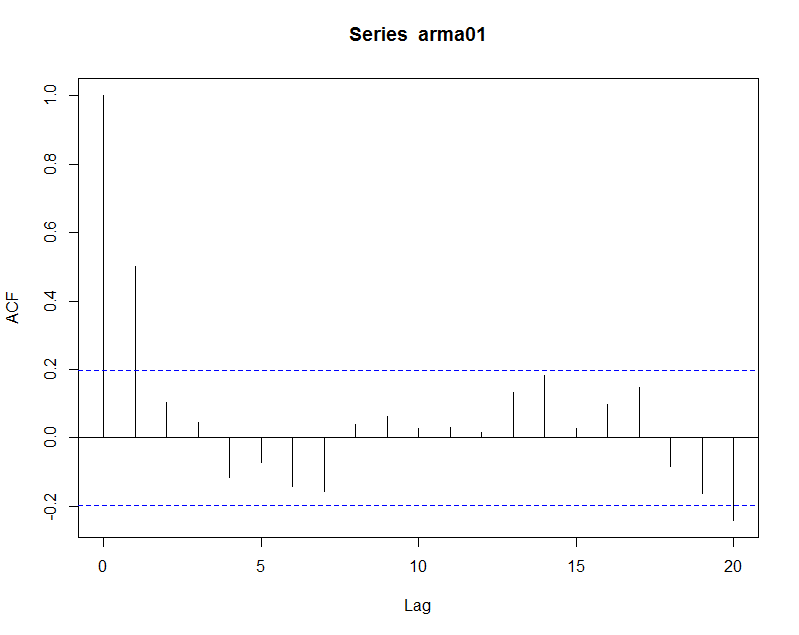
\includegraphics[width=5cm]{3.png}
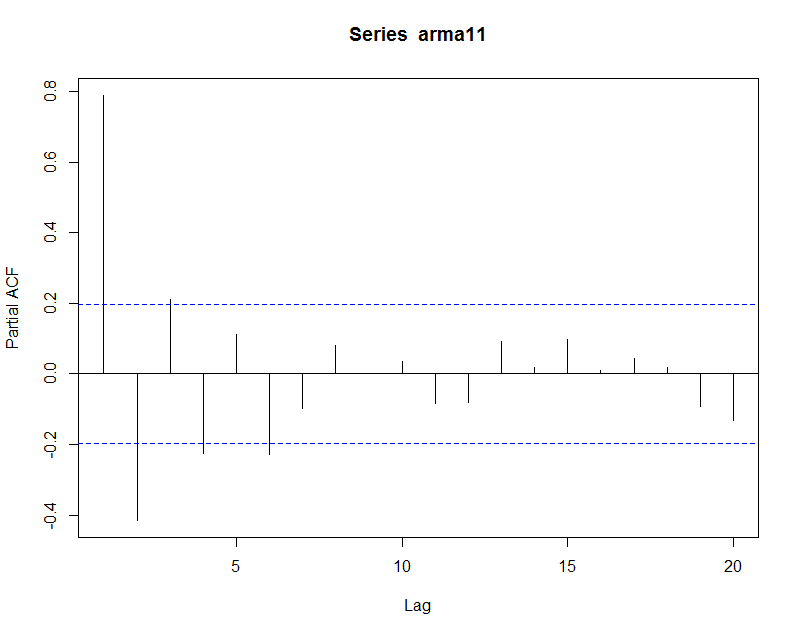
\includegraphics[width=5cm]{4.png}
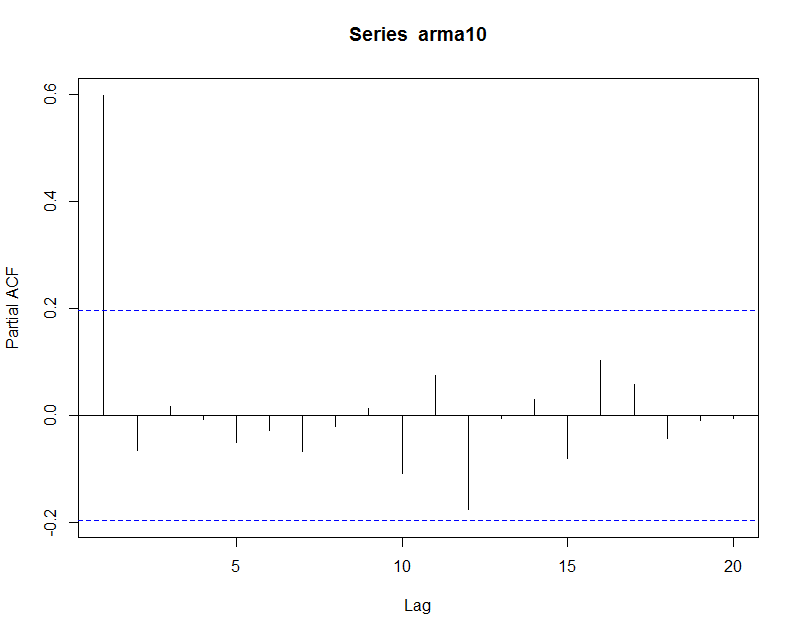
\includegraphics[width=5cm]{5.png}
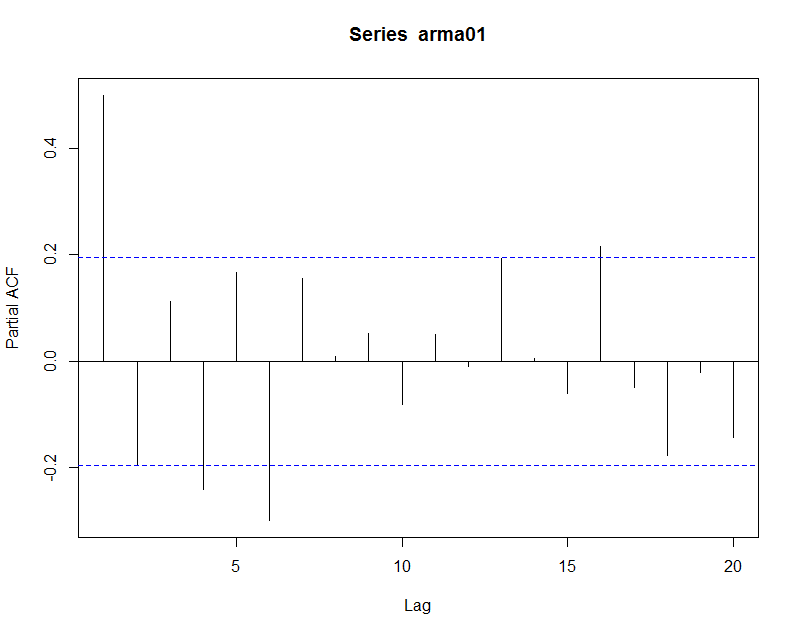
\includegraphics[width=5cm]{6.png}
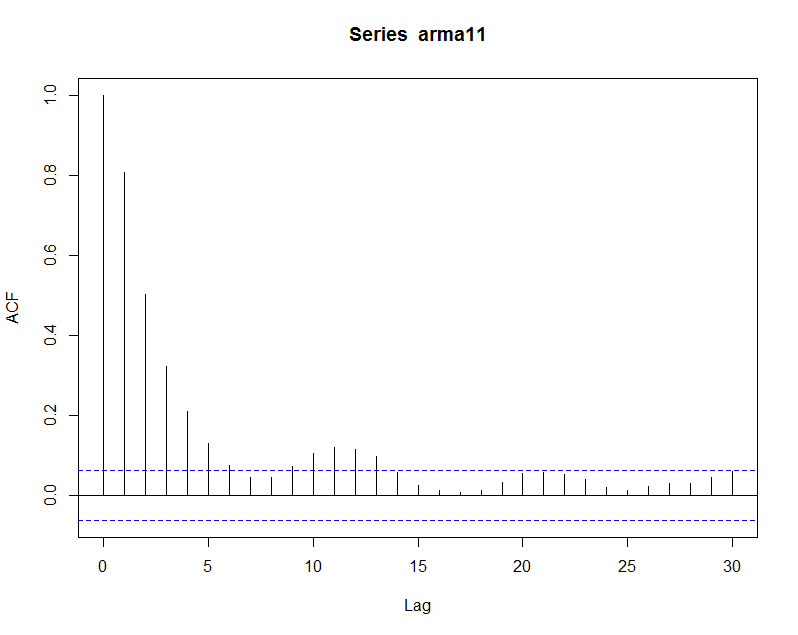
\includegraphics[width=5cm]{11.png}
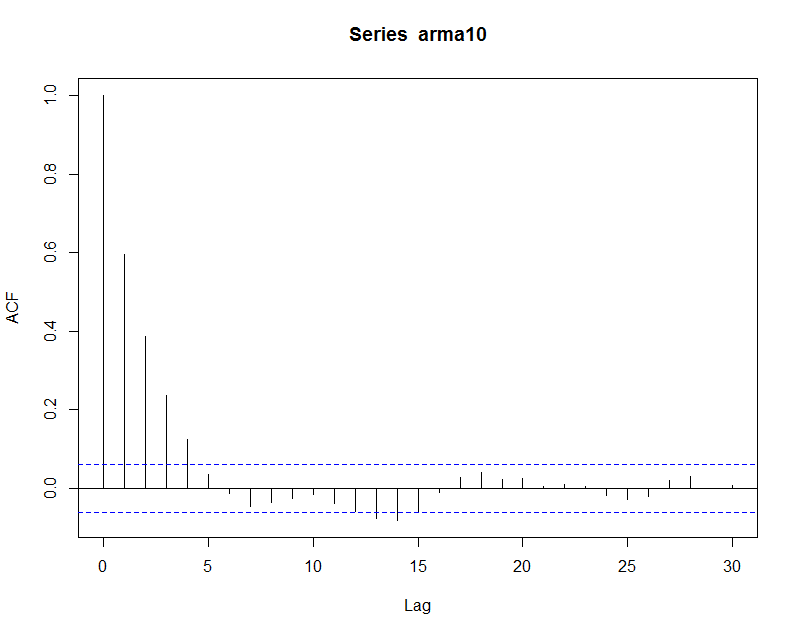
\includegraphics[width=5cm]{21.png}
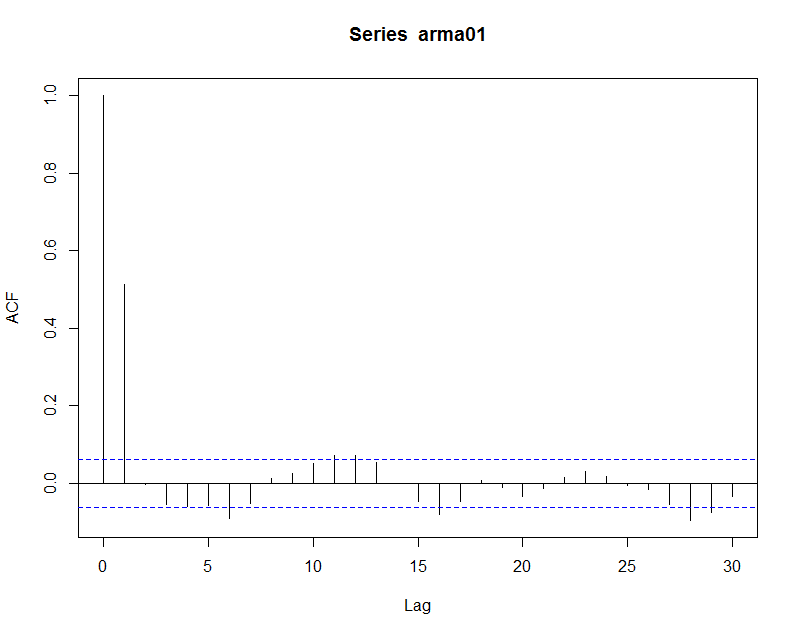
\includegraphics[width=5cm]{31.png}
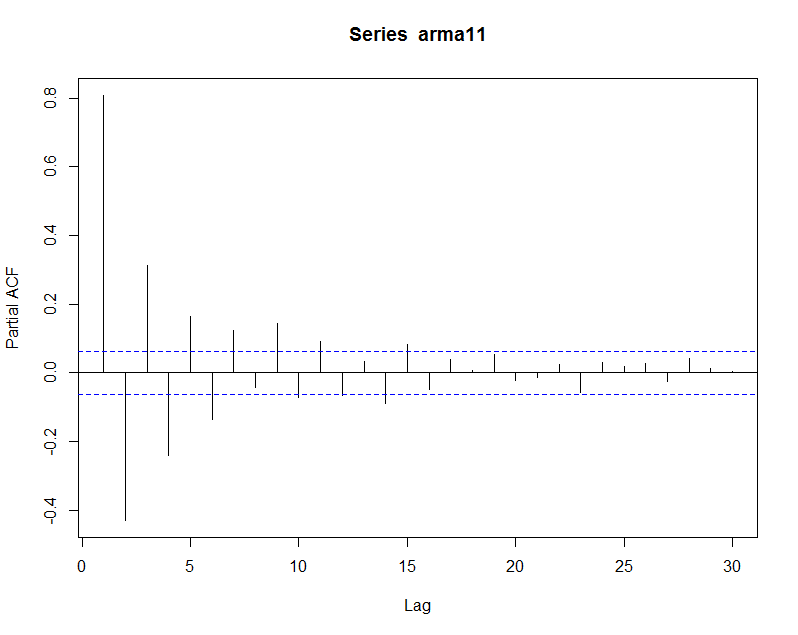
\includegraphics[width=5cm]{41.png}
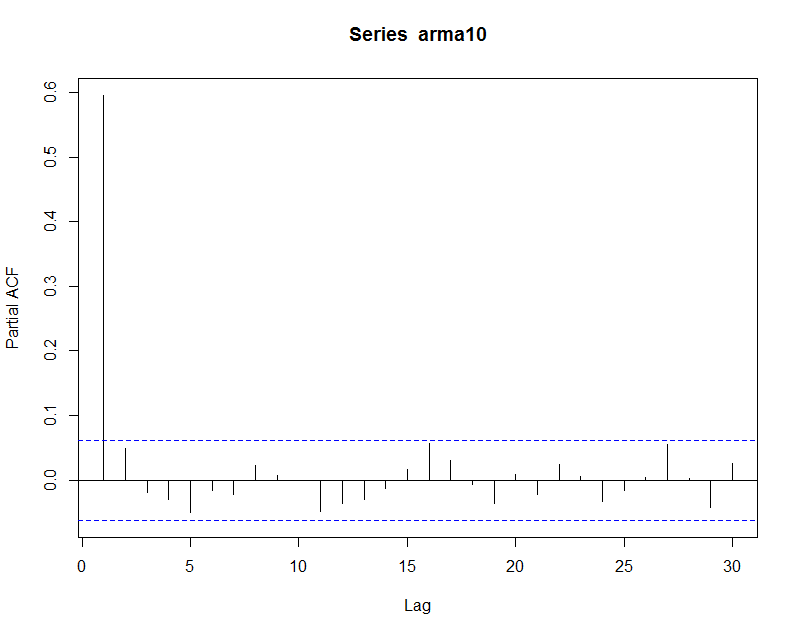
\includegraphics[width=5cm]{51.png}
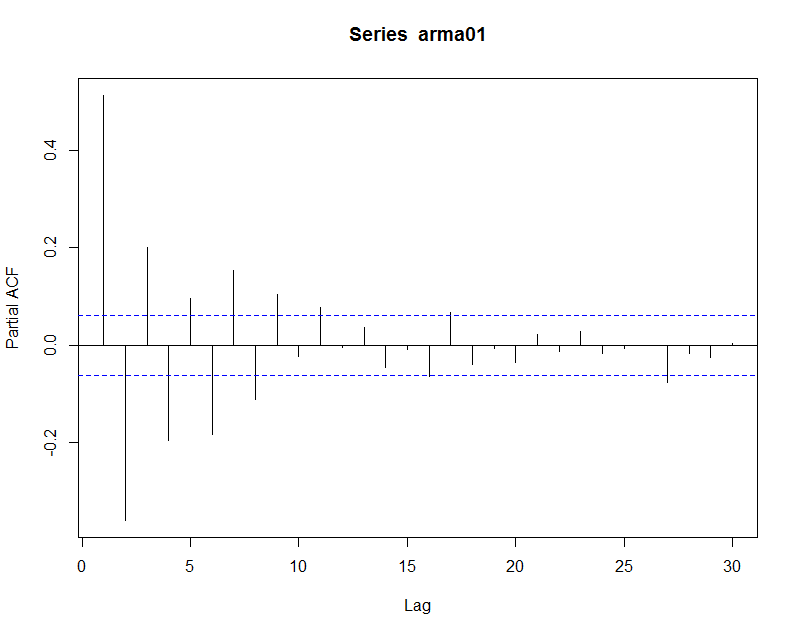
\includegraphics[width=5cm]{61.png}
\end{center}
\begin{lstlisting}[language=R,keywordstyle=\color{blue!70},commentstyle=\color{red!50!green!50!blue!50},frame=single,rulesepcolor=\color{red!20!green!20!blue!20},backgroundcolor=\color{backcolour},
]
#Problem 3.9

n = 1000
arma11 = arima.sim(n = n, list(ar = 0.6, ma = 0.9))
arma10 = arima.sim(n = n, list(ar = 0.6))
arma01 = arima.sim(n = n, list(ma = 0.9))

acf(arma11);acf(arma10);acf(arma01)

pacf(arma11);pacf(arma10);pacf(arma01)
\end{lstlisting}
\item[3.12]
\begin{align*}
    \ix{$\forall h>0$, by Cauchy Inequality,}
    |\gamma(h)|&=|\mbe{(x_0-\mu)(x_h-\mu)}|\\
    &\le \sqrt{\mbe{(x_0-\mu)^2}\mbe{(x_h-\mu)^2}}\\
    &= \gamma(0)\\
    \ix{The equation holds iff the distribution of $x_0$ and $x_h$ are equal. Since the pick of $x_0$ is alternative, if $\gamma(h)=\gamma(0)$, we can prove that for any positive integer $k$, $x_0=x_{kh}$, thus, }
    \gamma(kh)&= \gamma(0)> 0\\
    \ix{Let $k\rightarrow \infty$, it is contradict to $\gamma(h)\rightarrow 0$. Thus, $\forall h>0, |\gamma(h)|<\gamma(0)$. It means that $\Gamma$ is a strictly diagonally dominant matrix. So $|\Gamma|\ne 0$. By the proof of problem 1.25, the sample autocovariance is a non-negative definite funcition. So $\Gamma$ is positive semidefinite. Since $|\Gamma|\ne 0$,  $\Gamma$ is positive definite. }
\end{align*}
\item[3.14]
(a)\begin{align*}
	\argmin{g(x)}\mathrm{MSE}&=\argmin{g(x)}\int\left[\int (y-g(x))^2f(y|x)\dm y\right]f(x)\dx\\
    &=\argmin{g(x)}\int(y-g(x))^2f(y|x)\dm y\\
    &=\argmin{g(x)}\left(\mbe{y^2|x}-2\mbe{yg(x)|x}+\mbe{g^2(x)}\right)\\
    &=\mbe{y|x}\\
\ix{(b)}
	\mathrm{MSE}&=\mbe{(x^2+z-\mbe{x^2+z|x})^2}\\
    &=\mbe{z^2}\\
    &=1\\
\ix{(c)Apply $g(x)=a+bx$ to the function of \textrm{MSE},}
    \mathrm{MSE}&=\int\left[\int(y-a-bx)^2f(y|x)\dm y\right]f(x)\dx\\
    &=\mbe{\mbe{(y-bx)^2|x}-2a\mbe{y-bx|x}+a^2}\\
    &=\mbe{(y-bx)^2}-2a\mbe{y-bx}+a^2\\
    \argmin a \mathrm{MSE}&=\mbe{y-bx}=1\\
    \ix{thus,}
    \mathrm{MSE}&=\int\left[\int(y-1-bx)^2f(y|x)\dm y\right]f(x)\dx\\
    &=\mbe{\mbe{(y-1)^2|x}-2b\mbe{xy-x|x}+b^2x^2}\\
    &=b^2\mbe{x^2}-2b\mbe{xy-x}+\mbe{(y-1)^2}\\
    \argmin b&=\dfrac{\mbe{xy-x}}{\mbe{x^2}}\\
    &=\dfrac{\mbe{xy}}{\mbe{x^2}}=0\\
    \mathrm{MSE}&=\int\left[\int(y-1)^2f(y|x)\dm y\right]f(x)\dx\\
    &=\mbe{(x^2+z-1)^2}\\
    &=\mbe{x^4+z^2+1-2x^2}\\
    &=3+1+1-2=3
\end{align*}
Since $x$ has zero mean, the slope is zero, and the intercept equals to mean of y. MSE measures the variance of $y$.
In part (b), MSE measures the variance of $z$
\end{enumerate}
\end{CJK*}
\end{document}
